\documentclass[aspectratio=169,compress]{beamer}
\pdfpagewidth\paperwidth
\pdfpageheight\paperheight
\usepackage[greek,italian]{babel}
\usepackage[utf8]{inputenc}
\usepackage[T1]{fontenc}
\usepackage{lmodern,amsmath,amssymb,cclicenses,graphicx,apple_emoji,adjustbox}

\usetheme[background=light]{metropolis}%numbering=none
\useoutertheme{split}
\hypersetup{pdfstartview={Fit}} % fits the presentation to the window when first displayed

\metroset{block=fill}

\begin{document}
\title{Corso introduttivo a \LaTeX}
\subtitle{Lezione 2}
\author{Davide Peressoni}
\institute[]{Commissione Informatica\\Collegio Universitario don Nicola Mazza}
\date%[DATE CURTE]
{19 Dicembre 2018}
\titlegraphic{
\includegraphics[height=80px]{ComInfo}}

\setbeamertemplate{title page}{
  \begin{minipage}[b][\paperheight]{\textwidth}
    \vfill%
    \ifx\inserttitle\@empty\else\usebeamertemplate*{title}\fi
    \ifx\insertsubtitle\@empty\else\usebeamertemplate*{subtitle}\fi
    \usebeamertemplate*{title separator}
    \vspace*{1cm}
    \adjustbox{valign=M}{\ifx\inserttitlegraphic\@empty\else\usebeamertemplate*{title graphic}\fi}
    \adjustbox{valign=M}{\begin{minipage}{200px}
      \ifx\beamer@shortauthor\@empty\else\usebeamertemplate*{author}\fi
      \ifx\insertdate\@empty\else\usebeamertemplate*{date}\fi
      \ifx\insertinstitute\@empty\else\usebeamertemplate*{institute}\fi
    \end{minipage}}
    \vfill
    \vspace*{1mm}
  \end{minipage}
}
\setbeamertemplate{title graphic}{\inserttitlegraphic}

\maketitle

% \frame{\transfade
%   \frametitle{Table of Contents}
%   \tableofcontents[hideallsubsections]
% }
\frame{
  \tiny\cc 2018 Davide Peressoni\\~\par
    \emph{Le informazioni contenute nel presente docuemnto sono state verificate e documentate con la massima cura possibile. Nessuna responsabilità derivante dal loro utilizzo potrà venire imputata all’Autore coinvolto nella loro creazione, pubblicazione e distribuzione.}\\~\par
    Alcuni diritti riservati.\\~\\
    Documento prodotto con \LaTeX.\\
    Questo documento è rilasciato con licenza\\
    \begin{figure}[!ht]
	\centering
	    
\includegraphics{../Lezione1/CC.pdf}
    \end{figure}~\\
    \textbf{Creative Commons BY-NC-SA 4.0}\\
    Attribuzione – Non Commerciale - Stessa licenza\\
    \url{http://creativecommons.org/licenses/by-nc-sa/4.0/}\\
    \textbf{Attribuzione} — Devi riconoscere una menzione di paternità adeguata, fornire un link alla licenza e indicare se sono state effettuate delle modifiche. Puoi
    fare ciò in qualsiasi maniera ragionevole possibile, ma non con modalità tali da suggerire che il licenziante avalli te o il tuo utilizzo del materiale.\\
    \textbf{Non commerciale} — Non puoi usare il materiale per scopi commerciali.\\
    \textbf{Stessa licenza} — Se remixi, trasformi il materiale o ti basi su di esso, devi distribuire i tuoi contributi con la stessa licenza del materiale originario.
}

\section{Tabelle}
\begin{frame}[fragile]\transfade\centering
  \frametitle{Tabelle semplici}
\verb!\begin{tabular}{lc|r}                   !\\
\verb!  Nome        & Cognome & Età \\ \hline !\\
\verb!  Pinco Tizio & Pallino & 6 \\          !\\
\verb!  Mario       & Rossi   & 23            !\\
\verb!\end{tabular}                           !\\~\\
  \begin{tabular}{lc|r}
    Nome & Cognome & Età \\ \hline
    Pinco Tizio & Pallino & 6 \\
    Mario & Rossi & 23
  \end{tabular}\\~
\end{frame}
\begin{frame}[fragile]\transfade\centering
  \frametitle{Tabelle}
\verb!\begin{table}                       !\\
\verb!  \begin{tabular} ... \end{tabular} !\\
\verb!  \caption{Utenti del servizio}     !\\
\only<2->{\texttt{~~\textbackslash label\{tab:Utenti\}~~~~~~~~~~~~~~~~}\\}
\verb!\end{table}                         !\\
  \only<1>{\begin{table}
    \begin{tabular}{lc|r}
      Nome & Cognome & Età \\ \hline
      Pinco Tizio & Pallino & 6 \\
      Mario & Rossi & 23
    \end{tabular}
    \caption{Utenti del servizio}
    \label{tab:Utenti}
  \end{table}}
  \only<2->{~\\~\\~\texttt{come si evince dalla tabella \textbackslash ref\{tab:Utenti\} \textbackslash dots} \\Come si evince dalla tabella \ref{tab:Utenti} \dots}~\\
\end{frame}

\section{Immagini}
\begin{frame}\transfade\centering
  \frametitle{Immagini in linea}
\visible<3->{\texttt{\textbackslash usepackage\{graphicx\}}}\\
\texttt{\textbackslash includegraphics\only<4->{[width=300px,height=50px]}\{disegno\}}\\~\\
\only<2-3>{
\includegraphics[height=100px]{img/disegno}}
\only<4->{
\includegraphics[width=300px,height=50px]{img/disegno}}~\\~
\visible<5->{PDF, PNG e JPEG}
\end{frame}
\begin{frame}\transfade\centering
  \frametitle{Perché in linea?}
\texttt{Questa è \textbackslash includegraphics\{disegno\} una prova}\\~\\
\only<2->{Questa è 
\includegraphics[height=100px]{img/disegno} una prova}
\only<3->{\\Ciao {\footnotesize😀}, come va?}
\end{frame}

\begin{frame}[fragile]\transfade\centering
  \frametitle{Immagini}
  {\small\verb!\begin{figure}                       !\\
  \verb!  \includegraphics{immagine}         !\\
  \verb!  \caption{Disegno astratto}         !\\
  \only<2->{\texttt{~~\textbackslash label\{fig:Disegno\}~~~~~~~~~~~~~~~~}\\}
  \verb!\end{figure}                         !}
  \begin{figure}[!ht]%
    
\includegraphics[height=50px]{img/disegno}%
    \caption{Disegno astratto}%
    \label{fig:Disegno}%
  \end{figure}\vspace{-1.5em}%
  \only<2->{\small\texttt{Visibile in figura \textbackslash ref\{fig:Disegno\}} $\Rightarrow$ Visibile in figura \ref{fig:Disegno}\\~}
\end{frame}

\section{Riferimenti}
\frame{\transfade\centering
  \frametitle{Riferimenti}
  \texttt{Nel bel mezzo del cammin di nostra vita\textbackslash label\{ch:Prologo\}}\\~\\
  \visible<2->{\texttt{Come si legge nel capitolo \textbackslash ref\{ch:Prologo\} a pagina \textbackslash pageref\{ch:Prologo\}}}\\
  \visible<3->{Come si legge nel capitolo 1 a pagina 3}
}
\frame{\transfade\centering
  \frametitle{Tipi di riferimento}
  \begin{tabular}{l|l}
    prefisso & ambiente\\\hline
    ch: 	&chapter\\
    sec: 	&section\\
    subsec: 	&subsection\\
    fig: 	&figure\\
    tab: 	&table\\
    eq: 	&equation\\
  \end{tabular}
}
\begin{frame}[fragile]\transfade\centering
  \frametitle{Riferimenti ipertestuali}
  \verb!\usepackage[hidelinks]{hyperref}!\\~
\end{frame}

\section{Bibliografia}
\begin{frame}[fragile]\transfade\centering
  \frametitle{Bibliografia}
  \verb!\begin{thebibliography}{Numero massimo voci}               !\\
  \verb!  \addcontentsline{toc}{section}{Bibliografia}             !\\
  \verb!  \label{bibliografia}                                     !\\
  ~\\
  \verb!  \bibitem{WiFiStandard} %etichetta                        !\\
  \verb!    Ian Poole,\\                                           !\\
  \verb!    \emph{IEEE 802.11 Wi-Fi Standards},\\                  !\\
  \verb!    \url{http://www.radio.../ieee-802-11-standards.php},\\ !\\
  \verb!    consultato il 3 Giugno 2017.                           !\\
  ~\\
  \verb! \end{thebibliography}                                     !\\~
\end{frame}
\begin{frame}[fragile]\transfade\centering
  \frametitle{Richiami}
  \verb!... che utilizza modulazioni digitali \cite{WiFiStandard}!\\~\\~
  \visible<2->{... che utilizza modulazioni digitali~\cite{WiFiStandard}}\\~
  \only<3->{
    \begin{thebibliography}{8}
\setbeamertemplate{bibliography item}[text]
    \bibitem{WiFiStandard}
      Ian Poole,\\
      \emph{IEEE 802.11 Wi-Fi Standards},\\
      \url{http://www.radio-electronics.com/info/wireless/wi-fi/ieee-802-11-standards-tutorial.php},\\
      consultato il 3 Giugno 2017.
    \end{thebibliography}
  }
\end{frame}

\section{Inserire simboli}
\frame{\transfade\centering
  \frametitle{Siti}
  \begin{thebibliography}{8}
    \setbeamertemplate{bibliography item}[online]
    \bibitem{}
      Simboli matematici\\
      \url{https://en.wikibooks.org/wiki/LaTeX/Mathematics}
\\~\\~\\
    \setbeamertemplate{bibliography item}[article]
    \bibitem{}
      Tutti(?) i simboli\\
      \url{http://tug.ctan.org/info/symbols/comprehensive/symbols-a4.pdf}
    \end{thebibliography}
}
\frame{\transfade\centering
  \frametitle{Detextify}
  \url{http://detexify.kirelabs.org}
  \only<2->{~\\~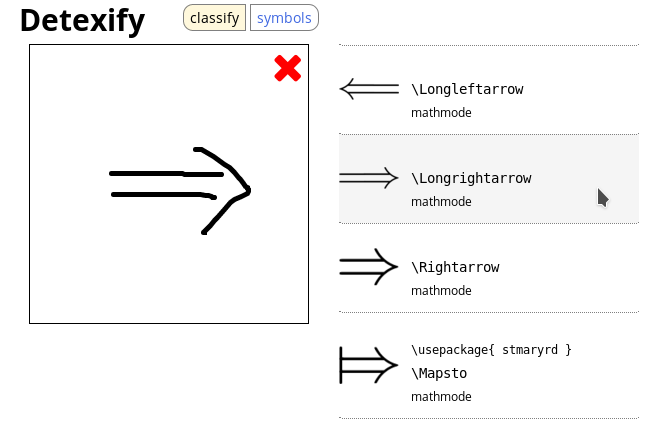
\includegraphics[height=0.7\paperheight]{img/detex}}
}

\appendix
\section{Scrivere in greco}
\begin{frame}[fragile]\transfade\centering
  \frametitle{Scrivere in greco}
  Nel preambolo: \verb!\usepackage[greek,italian]{babel}!\\
  Nel documento: \\
  \verb!\TeX~deriva dal greco \begin{otherlanguage}{greek}t'eqnh!\\
  \verb!\end{otherlanguage}~(arte, tecnica)!\\
  \visible<2->{\TeX~deriva dal greco \begin{otherlanguage}{greek}t'eqnh\end{otherlanguage}~(arte, tecnica)}\\~
\end{frame}

\setbeamercolor{background canvas}{bg=black}
\frame[plain]{\transfade}

\end{document}
